% Generated by pipeline/paper/scripts/make_result_figures.py. Do not edit by hand.
% First-run wall ratio versus stock. Four repeats, empty cache, new container. Not comparable to the EPYC savings node. Above 1 is slower than stock.
% Shared figure style. Input once; a second input is a no-op.
\ifdefined\actsplotsready
\else
  \def\actsplotsready{1}
  \colorlet{actsteal}{teal!72!black}
  \colorlet{actstealfaint}{teal!16}
  \colorlet{actsorange}{orange!88!black}
  \colorlet{actsink}{black!80}
  \colorlet{actsghost}{black!45}
  \colorlet{actsfail}{red!62!black}
  \colorlet{actsrule}{black!50}
  \usetikzlibrary{intersections}
  \usepgfplotslibrary{fillbetween,groupplots}
  \pgfplotsset{
    acts/.style={
      font=\scriptsize\sffamily,
      tick label style={font=\scriptsize\sffamily},
      label style={font=\scriptsize\sffamily},
      legend style={
        font=\scriptsize\sffamily,
        draw=none,
        fill=none,
        cells={anchor=west},
        inner sep=1pt,
        column sep=6pt
      },
      legend cell align=left,
      scale only axis,
      clip=false,
      axis line style={actsrule},
      tick style={actsrule},
      tick align=outside,
      axis lines=left,
      xmajorgrids=true,
      major grid style={black!7},
      ymajorgrids=false,
      every node/.append style={font=\scriptsize\sffamily, inner sep=1.5pt},
      every axis plot/.append style={line join=round, line cap=round},
    },
  }
  \tikzset{
    actlab/.style={
      font=\scriptsize\sffamily,
      fill=white,
      fill opacity=0.92,
      text opacity=1,
      inner sep=1.35pt,
      outer sep=0.5pt,
    },
  }
\fi

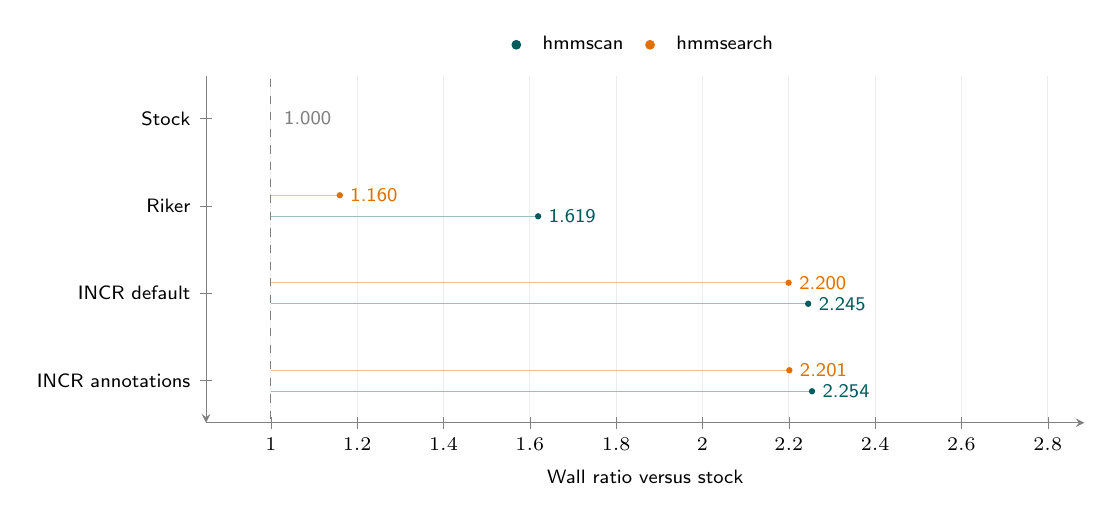
\begin{tikzpicture}
\begin{axis}[
  acts,
  width=0.92\columnwidth,
  height=4.4cm,
  xmin=0.85, xmax=2.88491,
  xlabel={Wall ratio versus stock},
  ytick={0,1,2,3},
  y dir=reverse,
  yticklabels={{Stock},{Riker},{INCR default},{INCR annotations}},
  enlarge y limits=0.16,
  legend style={at={(0.5,1.04)}, anchor=south, legend columns=2},
]
\addplot[draw=none, forget plot] coordinates {(1,0) (1,3)};
\addlegendimage{only marks, mark=*, mark size=1.55pt, draw=actsteal, fill=actsteal}
\addlegendentry{hmmscan}
\addlegendimage{only marks, mark=*, mark size=1.55pt, draw=actsorange, fill=actsorange}
\addlegendentry{hmmsearch}
% source: baseline_overhead.json modes.*.mean_paired_ratio
\draw[actsrule, dashed] (axis cs:1,-0.45) -- (axis cs:1,3.45);
\node[actlab, anchor=west, text=actsrule, xshift=3pt] at (axis cs:1,0) {1.000};
\draw[actsteal!40] (axis cs:1,1.12) -- (axis cs:1.6192894,1.12);
\fill[actsteal] (axis cs:1.6192894,1.12) circle[radius=1.15pt];
\node[actlab, anchor=west, text=actsteal, xshift=2pt] at (axis cs:1.6192894,1.12) {1.619};
\draw[actsorange!45] (axis cs:1,0.88) -- (axis cs:1.1598437,0.88);
\fill[actsorange] (axis cs:1.1598437,0.88) circle[radius=1.15pt];
\node[actlab, anchor=west, text=actsorange, xshift=2pt] at (axis cs:1.1598437,0.88) {1.160};
\draw[actsteal!40] (axis cs:1,2.12) -- (axis cs:2.2448942,2.12);
\fill[actsteal] (axis cs:2.2448942,2.12) circle[radius=1.15pt];
\node[actlab, anchor=west, text=actsteal, xshift=2pt] at (axis cs:2.2448942,2.12) {2.245};
\draw[actsorange!45] (axis cs:1,1.88) -- (axis cs:2.1995484,1.88);
\fill[actsorange] (axis cs:2.1995484,1.88) circle[radius=1.15pt];
\node[actlab, anchor=west, text=actsorange, xshift=2pt] at (axis cs:2.1995484,1.88) {2.200};
\draw[actsteal!40] (axis cs:1,3.12) -- (axis cs:2.253835,3.12);
\fill[actsteal] (axis cs:2.253835,3.12) circle[radius=1.15pt];
\node[actlab, anchor=west, text=actsteal, xshift=2pt] at (axis cs:2.253835,3.12) {2.254};
\draw[actsorange!45] (axis cs:1,2.88) -- (axis cs:2.2012595,2.88);
\fill[actsorange] (axis cs:2.2012595,2.88) circle[radius=1.15pt];
\node[actlab, anchor=west, text=actsorange, xshift=2pt] at (axis cs:2.2012595,2.88) {2.201};
\end{axis}
\end{tikzpicture}
